\documentclass{article}

\usepackage[utf8]{inputenc}
\usepackage{graphicx}
\usepackage{booktabs}
\usepackage{subcaption}
\usepackage{hyperref}
%\usepackage{biblatex}
\usepackage{wrapfig}

%\addbibresource{report.bib}

\title{A simple GPU ray tracer: Project report DD2360}
\author{Jacob Wahlgren \texttt{<jacobwah@kth.se>} \\ Expected grade: A}

\begin{document}

\maketitle

\section{Introduction}
% Background on the problem

Ray tracing is a 3D rendering technique enabling realistic optical effects by
simulating light rays. It is often used for visual effects and animation in film
and television. Using ray tracing is computationally expensive since a ray has
to be simulated for each pixel. However, since the rays are independent the
problem is embarrassingly parallel and easy to accelerate using GPUs.

A ray tracer casts a ray from the camera, through each pixel, into the scene.
The intersection points of the ray and all objects are computed and the point
closest to the camera is used to color the pixel. Material properties,
reflection angles, light sources etc are used to compute the final color.

\section{Methodology}
% Explain implementation

We used the Blinn-Phong shading model, where the color $C$ at an intersection
point is given by the following formula. Let $C_a$ be the ambient color, $D$
the amount of diffuse lighting, $N$ the normal, $L$ a normal vector pointing to
the light source, $C_m$ the material color, $c$ the amount of specular lighting, $C_l$ the color of the
light source, $H$ the normal vector halfway vector between the ray and the light
source, and $k$ the specular exponent.
\begin{equation}
    C = C_a + C_m \cdot D \cdot \max\{(N, L), 0\} + C_l \cdot c \cdot \max\{(H, N),
    0\}^k
\end{equation}
We render a scene with a single light source and a single solid sphere. The
resulting image is written to a file in the PPM format using 3 bytes per pixel.
Each pixel is computed by one thread in square tile blocks of configurable
size.

The kernel is similar to the Python code in structure and content. The thread
and block indices are used to calculate the pixel coordinates. Operator
overloading on the \verb|float3| type is used to simplify vector operations. The
color is computed in $[0,1]$ float space and at the end converted to $[0,255]$
int space.

Since the task is IO bound, we investigate three different techniques for
writing the image to file. The \textbf{fwrite} version is the simplest, where
the whole image is rendered, then copied to RAM, and then written to file with a
single write call. The \textbf{mmap} version truncates the file to the output
size and then memory maps the whole file. Once the image is rendered it is
copied directly into the memory mapped file. The \textbf{streams} version uses
multiple overlapping streams to render, copy, and write chunks of the image in
parallel. Each chunk corresponds to a horizontal line of blocks in the image.

The code is available at \url{https://github.com/jacwah/cuda-raytracer}.

\section{Experimental setup}
% Gpu platform, software and hardware, tools

Experiments are run on the Tegner cluster at the PDC Center for High Performance
Computing at KTH. These nodes have two 12 core Intel E5-2690v3 Haswell
processors with 512 GB RAM. Files are written to a parallel Lustre file system.
The performance is evaluated both on nodes with NVIDIA Quadro K240 and the
NVIDIA Tesla K80. The GPUs are programmed using CUDA.

The reference CPU implementation in Python was modified to call \verb|savefig|
to write the image to a file instead of displaying it interactively.

\begin{wrapfigure}{r}{0.5\linewidth}
    %\centering
    \includegraphics{../fig/cpu.pdf}
    \caption{Comparison between Python CPU and fwrite 8x8
    GPU, average of 10 runs, on Tegner thin node.}
    \label{fig:cpu}
\end{wrapfigure}

\section{Results}
% Validation, performance

\begin{table}
    \centering
    \begin{tabular}{@{}llc@{}}
        \toprule
        GPU & Implementation & Execution time (s) \\
        \midrule
        NVIDIA Quadro K240 & streams (pinned) & $0.95 \pm 0.38$ \\
        NVIDIA Tesla K80 & fwrite (pinned) & $1.32 \pm 0.48$ \\
        \bottomrule
    \end{tabular}
    \caption{Fastest configurations at 10,000x10,000 pixels.}
    \label{tab:fast}
\end{table}

Visual inspection of the generated images using the \verb|display| command
validated the results. For the largest image size ImageMagick was used to resize
the image before viewing. Example images are shown in figure \ref{fig:output}.

The performance comparison of the CPU and GPU versions showed that the GPU
vastly outperforms the CPU version on this task. The difference was more
noticeable at larger image dimensions. In fact, results were not obtained for
the CPU version above image dimension 1000 since it was too slow. The results
are presented in figure \ref{fig:cpu}, were the Quadra K240 fwrite 8x8
configuration is used to represent the GPU.

We evaluate the performance of different GPU configurations at image size
1000x1000 (normal) and 10,000x10,000 (huge). The image files are 3 MB and 287
MB respectively.

At the normal image size, all
configurations perform similarly to each other. The K240 is
consistently faster. Figure \ref{fig:1000} shows the results for all
configurations.

At the huge image size, the results were more varied. On the Quadro K240 the
fastest configurations were streams (pinned) with 8x8 or larger block size. Also
close were fwrite (pinned) with 8x8 block size. On the Tesla K80 the fastest
configuration was fwrite (pinned) 16x16. Also close were regular fwrite 16x16
and streams 8x8 and 16x16. The execution time of the fastest configurations are
presented in table \ref{tab:fast}. Figure \ref{fig:10000} shows the results for
all configurations.

\begin{figure}
    \begin{subfigure}{0.5\linewidth}
        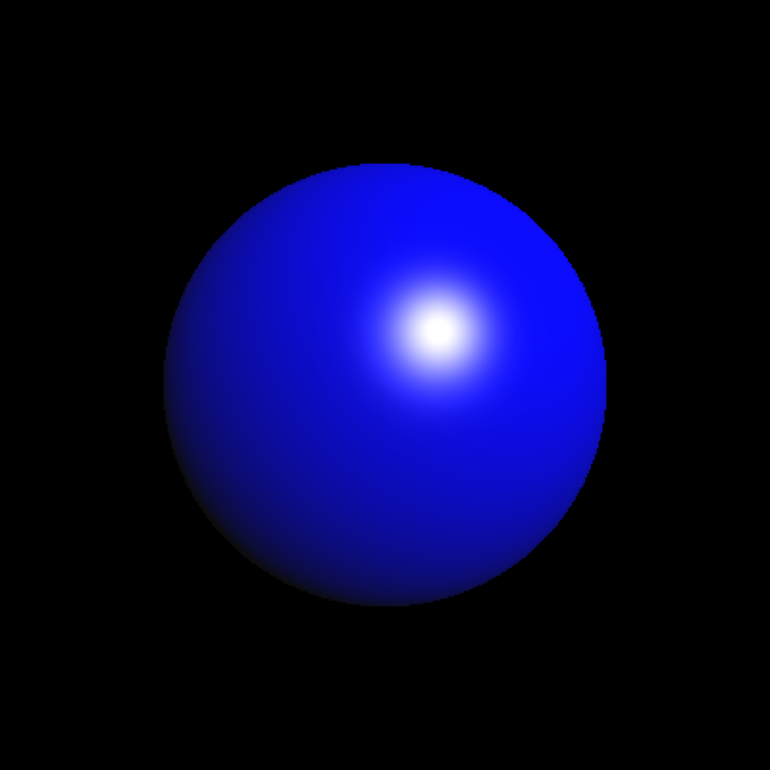
\includegraphics[width=\linewidth]{../raytracing_py_trim.png}
        \caption{CPU}
    \end{subfigure}
    \begin{subfigure}{0.5\linewidth}
        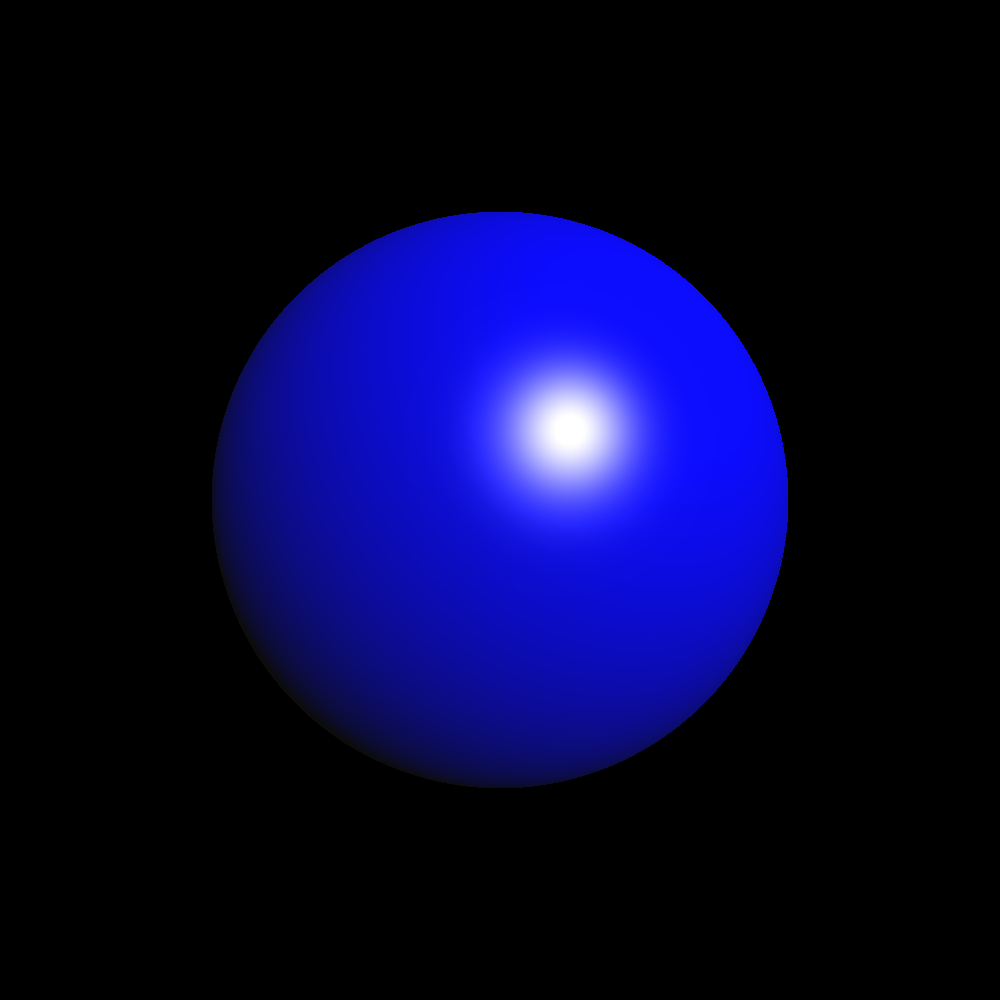
\includegraphics[width=\linewidth]{output.png}
        \caption{GPU}
    \end{subfigure}
    \caption{Sample output images.}
    \label{fig:output}
\end{figure}

\section{Discussion and conclusion}
% Discuss performance results
% Challenges and limitations
% Optimizations

The massive parallelism offered by the GPU vastly outperforms the reference CPU
implementation. However, a more fair comparison would use a faster language than
Python and utilize all the available compute power of the CPU rather than a
single thread.

The specular highlight in output images from the CPU and the GPU versions are
slightly different. This is likely caused by using different floating
point precision (double in Python, single in CUDA).

When it comes to comparing the various GPU implementations, the differences at a
normal image size of 1000x1000 pixels are negligible. The reason could be that a
configuration independent overhead, such as initializing the CUDA context,
dominates the run time.

In contrast, for the huge image size of 10,000x10,000 pixels the differences
are very large. The various implementations perform differently on the two GPUs
used. On the K240 usage of pinned memory clearly improves the results for
fwrite and streams which both perform well. On the K80 fwrite performs well both
with and without pinned memory, while streams performs well only without pinned
memory.

The mmap
implementation has very large variations in run time, and is overall the
slowest. The results indicate that the overhead of memory mapping is not worth
it, since each byte is only
accessed once.
In the words of Linus Torvalds, ``playing games with the virtual memory mapping
is very expensive in
itself''\footnote{\url{https://yarchive.net/comp/mmap.html\#6}}.

In conclusion, ray tracing is a task that can greatly benefit from GPU
acceleration. Depending on which GPU is used various techniques can be used to
reduce IO cost.

Future work could investigate how the streams implementation can be tweaked to
increase performance. What chunk sizes and number of streams are optimal? Why
does the pinned version perform poorly on the K80? On a parallel file system, is
it better to buffer the writes?

A more complex scene and shading model could also change the performance
characteristics, since the computation would occupy a larger fraction of the run time.
How would this change the behavior of the different implementations?

%\printbibliography

\begin{figure}
    \begin{subfigure}{\linewidth}
        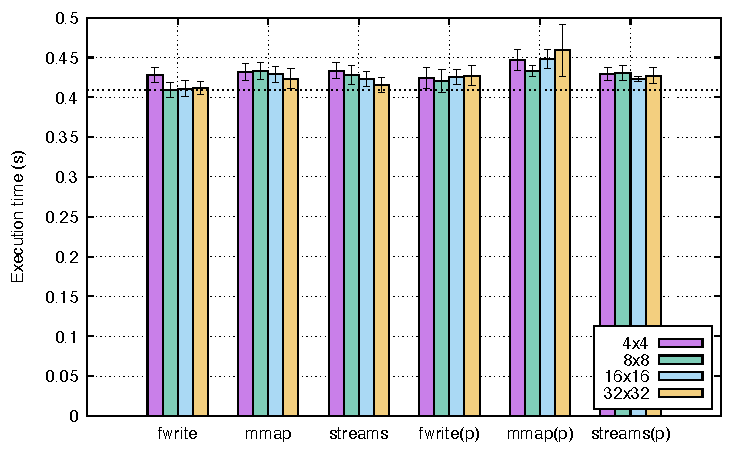
\includegraphics{../fig/sm30-1000.pdf}
        \caption{NVIDIA Quadro K240}
    \end{subfigure}
    \begin{subfigure}{\linewidth}
        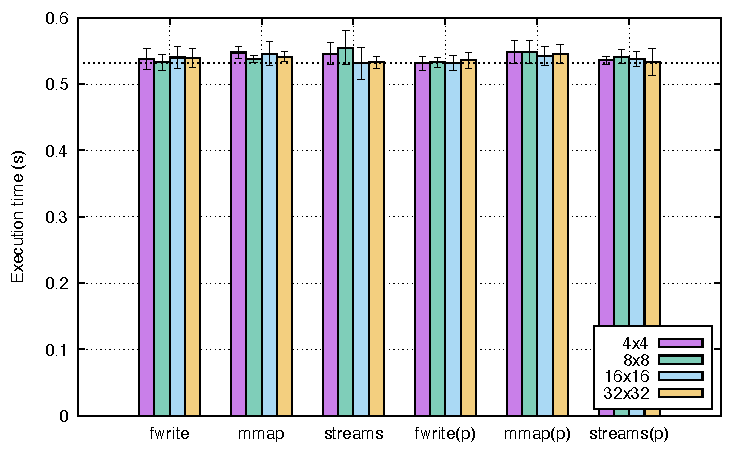
\includegraphics{../fig/sm37-1000.pdf}
        \caption{NVIDIA Tesla K80}
    \end{subfigure}
    \caption{Performance results for 1000x1000 image with various block sizes.
        Bars show average, whiskers show standard deviation. Usage of pinned
    memory is indicated by (p). The black dotted line shows the minimum value.}
    \label{fig:1000}
\end{figure}

\begin{figure}
    \begin{subfigure}{\linewidth}
        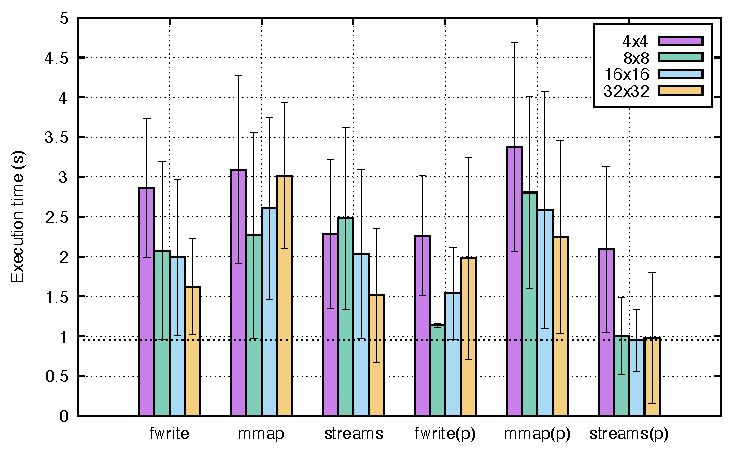
\includegraphics{../fig/sm30-10000.pdf}
        \caption{NVIDIA Quadro K240}
    \end{subfigure}
    \begin{subfigure}{\linewidth}
        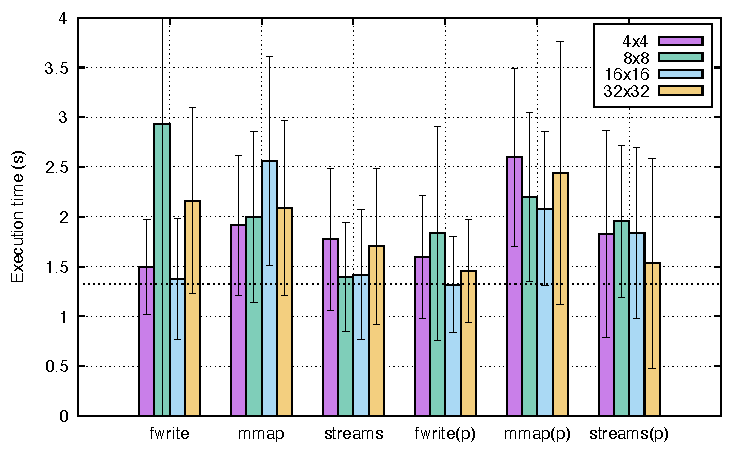
\includegraphics{../fig/sm37-10000.pdf}
        \caption{NVIDIA Tesla K80}
    \end{subfigure}
    \caption{Performance results for 10,000x10,000 image with various block
    sizes. Bars show average, whiskers show standard deviation. Usage of pinned
    memory is indicated by (p). The black dotted line show the minimum value.}
    \label{fig:10000}
\end{figure}

\end{document}
